\documentclass[12pt]{article}

\usepackage[a4paper, margin=2.5cm]{geometry}
\usepackage{amsmath}
\usepackage{booktabs}
\usepackage{array}
\usepackage{multirow}
\usepackage{parskip}
\usepackage{setspace}
\usepackage{microtype}
\usepackage{float}
\usepackage{graphicx}
\usepackage{hyperref}
\usepackage[T1]{fontenc}
\usepackage[utf8]{inputenc}

\setlength{\parindent}{1.5em}
\setlength{\parskip}{0pt}
\onehalfspacing

\hypersetup{
    colorlinks=true,
    urlcolor=black,
    linkcolor=black
}

\begin{document}

%% ---------------------------------------------------------------
%%  TITLE PAGE
%% ---------------------------------------------------------------
\begin{titlepage}
    \centering
    \vspace*{3cm}

    {\LARGE \textbf{Explainable NLP for Caption Similarity and
    Hashtag Recommendation}}\\[1.2em]
    {\large Results (NLP Course)}

    \vspace{3cm}

    \textbf{Group:} A\\[0.8em]

    \textbf{Students:}\\
    Juan Sebastian Pe\~na\\
    Saad Ayomide Olowolayemo\\[0.8em]

    \textbf{Instructor:}\\
    Juan Jos\'e Manjar\'in Colon

    \vfill

    {\large April 2026}
\end{titlepage}

%% ---------------------------------------------------------------
%%  RESULTS
%% ---------------------------------------------------------------
\section*{Results}

\setlength{\parindent}{1.5em}

An initial dataset of 26,623 raw TikTok posts was retrieved from a
PostgreSQL database hosted on Supabase, collected via a custom scraper
available at \url{https://github.com/PredictiveSocialMedia/Tik-Tok-Recommendation-System}.
During preprocessing, 3,976 posts (14.9\%) were excluded for having fewer
than four non-hashtag characters, leaving a final dataset of 22,647 posts.
All four engagement variables (likes, comments, views, shares) were
log-transformed using $y' = \log(1 + y)$ to reduce skew. Labels were
assigned via a median split of log-transformed view counts (median = 13.06),
yielding 11,324 high-engagement and 11,323 low-engagement posts and a 50\%
baseline accuracy for classifier evaluation.

Two complementary text representations were developed: a TF-IDF matrix
($22{,}647 \times 10{,}000$, density 0.16\%) capturing lexical patterns,
and 384-dimensional SBERT embeddings (\texttt{all-MiniLM-L6-v2}) capturing
semantic meaning. To validate the embeddings, UMAP reduced the space to two
dimensions (Figure~\ref{fig:umap}). The projection shows a dense central
region with scattered outliers, typical of a short-text corpus with high
topical diversity. High- and low-engagement posts intermix throughout the
space without clear separation, consistent with the classification results
reported below.

\begin{figure}[H]
    \centering
    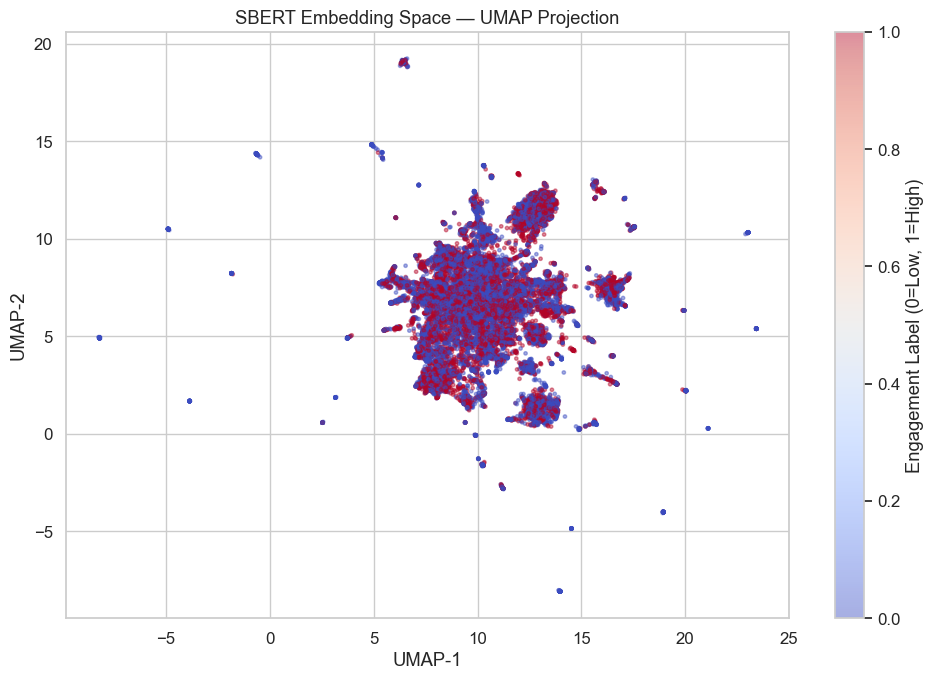
\includegraphics[width=0.52\textwidth]{figures/fig_umap.png}
    \caption{UMAP projection of SBERT caption embeddings. High- (red) and
    low-engagement (blue) posts intermix throughout, confirming that
    semantic similarity does not separate by engagement level.}
    \label{fig:umap}
\end{figure}

Four classifiers were trained on 80\% of the data and evaluated on a
stratified held-out set of 4,530 posts: Logistic Regression (SBERT),
Multinomial Na\"ive Bayes (TF-IDF), and KNN with SBERT for
$k \in \{5, 10\}$.
All models achieved comparable overall performance (59--60\% accuracy,
macro F1 0.58--0.59), yet the per-class breakdown in
Table~\ref{tab:classification} reveals meaningful differences. Na\"ive
Bayes heavily favoured high-engagement recall (0.79) at the cost of
low-engagement recall (0.41), reflecting a bias toward vocabulary common
in popular posts. KNN at $k=10$ showed the inverse pattern. Logistic
Regression maintained the most balanced trade-off and is the most reliable
baseline overall. Figure~\ref{fig:cm} makes the asymmetries visually
apparent. The consistent accuracy ceiling across both lexical and semantic
representations suggests the bottleneck is the information content of
captions themselves: on TikTok, engagement is driven predominantly by
non-textual factors such as audio, visuals, and platform algorithms.

\begin{table}[H]
    \centering
    \caption{Per-class classification results (test set, $n = 4{,}530$).}
    \label{tab:classification}
    \setlength{\tabcolsep}{6pt}
    \begin{tabular}{llcccccc}
        \toprule
        & & \multicolumn{3}{c}{\textbf{Low engagement}}
          & \multicolumn{3}{c}{\textbf{High engagement}} \\
        \cmidrule(lr){3-5}\cmidrule(lr){6-8}
        \textbf{Model} & \textbf{Features} & P & R & F1 & P & R & F1 \\
        \midrule
        Logistic Regression       & SBERT  & 0.60 & 0.59 & 0.59 & 0.59 & 0.60 & 0.60 \\
        Multinomial Na\"ive Bayes & TF-IDF & 0.66 & 0.41 & 0.50 & 0.57 & 0.79 & 0.66 \\
        KNN ($k=5$)               & SBERT  & 0.58 & 0.63 & 0.61 & 0.60 & 0.54 & 0.57 \\
        KNN ($k=10$)              & SBERT  & 0.57 & 0.73 & 0.64 & 0.62 & 0.44 & 0.51 \\
        \bottomrule
    \end{tabular}
\end{table}

\begin{figure}[H]
    \centering
    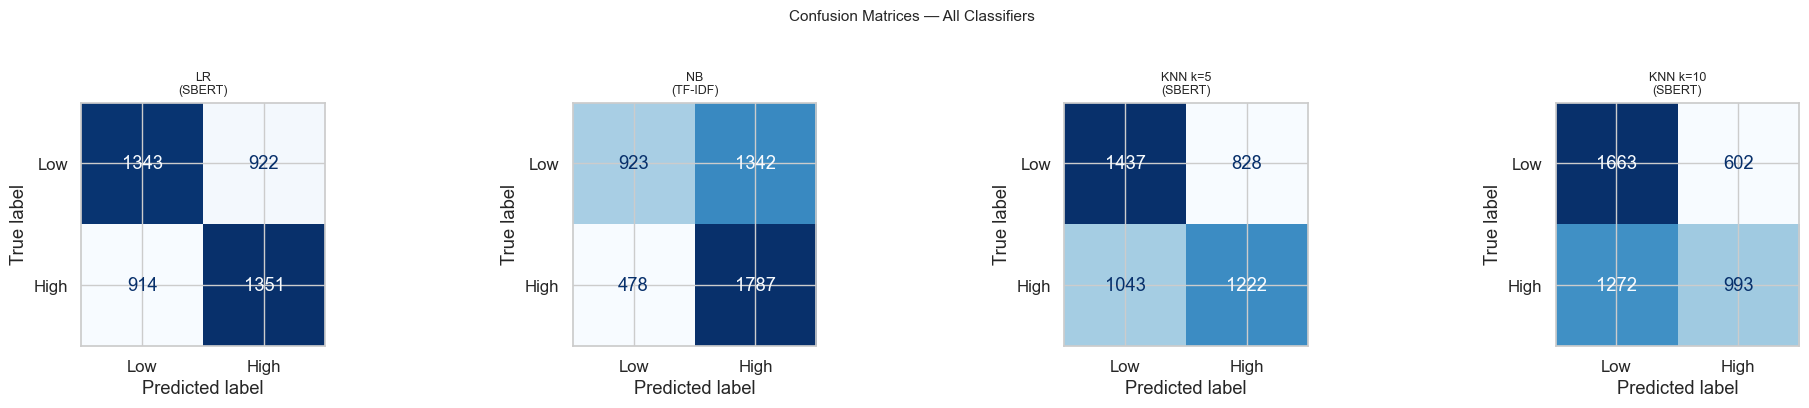
\includegraphics[width=\textwidth]{figures/fig_confusion_matrices.png}
    \caption{Confusion matrices for all four classifiers (test set,
    $n = 4{,}530$). Class~0 = low engagement; Class~1 = high engagement.}
    \label{fig:cm}
\end{figure}

For each of the 22,647 posts, semantic neighborhoods were constructed using
cosine similarity in the SBERT embedding space at three sizes
($K = 5, 10, 20$). Within each neighborhood, the variance of the four
log-transformed engagement metrics was compared to a null distribution from
1,000 random groups of the same size. All twelve variance reduction values
were positive, ranging from 10.46\% to 13.04\% (Table~\ref{tab:variance}),
and one-sided Mann-Whitney U tests returned $p \approx 0.0$ in every case,
confirming the result is not due to chance. Variance reduction decreased
steadily with neighborhood size --- from $\approx$12.6\% at $K=5$ to
$\approx$10.9\% at $K=20$ --- as larger groups incorporate more topically
diverse posts. Levene's test added nuance: at $K=5$ the effect mainly
reflects a shift in central tendency ($p > 0.05$ for all metrics), whereas
at $K=10$ and $K=20$ significant differences in dispersion emerged, showing
structural contrasts grow more pronounced at larger scales.

\begin{table}[H]
    \centering
    \caption{Variance reduction (\%) of semantic vs.\ random neighborhoods.
    All twelve Mann-Whitney U tests: $p \approx 0.0$.}
    \label{tab:variance}
    \begin{tabular}{lcccc}
        \toprule
        $K$ & \textbf{likes\_log} & \textbf{comments\_log}
        & \textbf{views\_log} & \textbf{shares\_log} \\
        \midrule
        5  & 13.04\% & 12.72\% & 12.32\% & 12.46\% \\
        10 & 12.30\% & 12.74\% & 11.36\% & 11.98\% \\
        20 & 11.34\% & 11.27\% & 10.46\% & 10.53\% \\
        \bottomrule
    \end{tabular}
\end{table}

A secondary finding concerns hashtag coverage. Initially only 883 posts
(3.9\%) contained hashtags in the bridge-table field. By also extracting
hashtags from caption text, coverage reached 100\% --- an average of 5.58
tags per post across 36,866 unique tags. Recommendations are generated by
aggregating hashtags from the $K$ nearest semantic neighbors and ranking
them by frequency and average log-engagement. Table~\ref{tab:recs} shows
results for three unseen captions at inference time; across fitness,
finance, and food verticals, the top-ranked hashtags consistently matched
the topic and tone of each query. Every recommendation traces to a specific corpus post, making the system
interpretable.

\begin{table}[H]
    \centering
    \caption{Top hashtag recommendations for three unseen captions.
    Freq.\ = occurrences among $K$ nearest neighbors.}
    \label{tab:recs}
    \setlength{\tabcolsep}{8pt}
    \begin{tabular}{p{5.8cm} p{3.8cm} c c}
        \toprule
        \textbf{Query caption} & \textbf{Hashtag} & \textbf{Freq.} & \textbf{Avg.\ log-eng.} \\
        \midrule
        \multirow{3}{5.8cm}{\textit{``Just hit a new personal record at the gym! Hard work always pays off''}}
            & \#fitness    & 7 & 14.2 \\
            & \#gymtok     & 4 & 13.8 \\
            & \#gym        & 3 & 13.5 \\
        \midrule
        \multirow{3}{5.8cm}{\textit{``Crypto market update --- here is my honest take on what is happening right now''}}
            & \#stockmarket    & 6 & 13.1 \\
            & \#cryptocurrency & 4 & 12.9 \\
            & \#crypto         & 3 & 12.7 \\
        \midrule
        \multirow{3}{5.8cm}{\textit{``Healthy high-protein meal prep for the week, my go-to lunch routine''}}
            & \#highprotein      & 3 & 13.4 \\
            & \#mealprepideas    & 2 & 12.8 \\
            & \#highproteinmeals & 2 & 12.6 \\
        \bottomrule
    \end{tabular}
\end{table}

Several limitations must be acknowledged. Caption text captures only part
of what drives engagement, as the 59--60\% accuracy ceiling makes clear.
The SBERT model was trained predominantly on English, so performance may
degrade on slang or mixed-language captions. Variance reduction varies with
$K$ (10.5\%--13.0\%), requiring calibration to the desired precision--recall
trade-off. The dataset is also a static snapshot; the KNN index cannot
absorb new posts without a full rebuild. Future work could address these
constraints through multilingual models, incremental indexing, and the
incorporation of multimodal signals to push engagement prediction beyond
the current ceiling.

\end{document}
